% -*- root: ../main.tex -*-

\documentclass[../main.tex]{subfiles}
\begin{document}

\chapter{Reduzierte-Basis-Methode} % (fold)
\label{chapter:rbm}

% chapter reduzierte_basis_methode (end)

Nun wird aufbauend auf das Petrov-Galerkin-Verfahren des vorherigen Kapitels die Reduzierte-Basis-Methode eingeführt und auf das gegebene Setting übertragen.
Anschließend wird die numerische Umsetzung dieser für unsere bereits in \cref{section:galerkin_numerische_umsetzung_und_experimente} betrachtete Problemstellung angegangen und die Ergebnisse diskutiert.

\section{Grundlagen} % (fold)
\label{sub:grb:rb:grundlagen}

Wir beginnen mit einer kurzen Motivation und Einführung der Reduzierte"=Basis"=Methoden.
Dabei handelt es sich um ein relativ junges Verfahren, welches besonders in den letzten Jahren viel Aufmerksamkeit und Weiterentwicklung erfahren hat.
Eine weitaus umfassendere Einführung als die nachfolgende findet man beispielsweise in der Arbeit von \textcite{Patera:2007un}.

Um die Idee hinter der Reduzierte-Basis-Methode zu erklären, benötigen wir das folgende Setting: Sei $\mathcal P \subset \mathbb{R}^{p}$ eine abgeschlossene und konvexe Parametermenge und sei das folgende parametrische Variationsproblem gegeben:
Sei $\mu \in \mathcal P$, finde $u(\mu) \in \mathcal X$ mit
\begin{equation}
    \label{eq:rbm_varprob_allgemein}
    b(u(\mu), v; \mu) = f(v; \mu) \quad \fa v \in \mathcal Y,
\end{equation}
wobei $b(\blank, \blank; \mu) \colon \mathcal X \times \mathcal Y \to \mathbb{R}$ eine Bilinearform und $f(\blank; \mu) \colon \mathcal Y \to \mathbb{R}$ ein lineares Funktional ist, so dass für alle $\mu \in \mathcal P$ das obige Variationsproblem korrekt gestellt ist.
Probleme dieser Art werden oft, wie beispielsweise in \cref{chapter:galerkin} beschrieben, mittels Galerkin-Verfahren auf hochdimensionalen Räumen $\mathcal X_{\mathcal N}$ und $\mathcal Y_{\mathcal N}$ gelöst.
Wir stützen uns darauf, dass der Fehler dieser Diskretisierung theoretisch beliebig klein gehalten werden kann und bezeichnen im Folgenden die Räume $\mathcal X_{\mathcal N}$ und $\mathcal Y_{\mathcal N}$ als Truth-Ansatz- respektive Truth-Testraum und die entsprechende diskrete Lösung $u_{\mathcal N}(\mu) \in \mathcal X_{\mathcal N}$ als Truth-Lösung.

Unter der Annahme, dass die Lösung $u(\mu) \in \mathcal X$ eine gewissen Regularität bezüglich des Parameters $\mu \in \mathcal P$ aufweist, hat die durch die Lösungen gebildete Mannigfaltigkeit $\mathcal M_{\mathcal N} = \Set{u_{\mathcal N}(\mu) \in \mathcal X_{\mathcal N} \given \mu \in \mathcal P}$ meist eine eher niedrige Dimension, vergleiche \cref{fig:figure1}.
Hier setzen die Reduzierte-Basis-Methoden an; der Reduzierte-Basis-Ansatzraum $\mathcal X_{N}$ wird definiert als $N$-dimensionale Approximation
\begin{equation}
    \mathcal X_{N} = \spn\Set{u_{\mathcal N}(\mu_{i}) \given i = 1 \dots N} = \spn\Set{\xi_{1}, \dots, \xi_{N}}
\end{equation}
an $\mathcal M_{\mathcal N}$, wobei $N \ll \mathcal N$ wünschenswert ist.
Die Reduzierte-Basis-Lösung $u_{N}(\mu)$ wird dann durch erneute Galerkin-Projektion von \cref{eq:rbm_varprob_allgemein} auf $\mathcal X_{N}$ und einen noch näher zu bestimmenden Reduzierte-Basis-Testraum $\mathcal Y_{N}$ bestimmt.

\begin{figure}[tb]
    \centering
    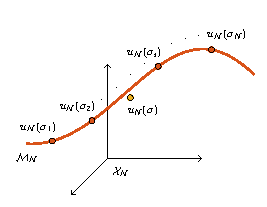
\includegraphics[width=0.6\textwidth]{figures/rb.pdf}
    \caption[%
    Skizze zur Motivation der Reduzierte-Basis-Methode.
    ]{
        Skizzenhafte Darstellung der Funktionsweise der Reduzierte-Basis-Methode.
        Die Reduzierte-Basis-Approximation $u_{N}(\mu)$ ergibt sich als Linearkombination der Finite-Elemente-Snapshots $u_{\mathcal N}(\mu_{i})$, welche mutmaßlich eine glatte parametrische Manigfaltigkeit bilden.
        }
    \label{fig:figure1}
\end{figure}


\section{Grundlagen pt. II} % (fold)
\label{sec:grundlagen}

Wir knüpfen an \cref{chapter:galerkin} an und betrachten zunächst ein abstraktes parametrisches Variationsproblem der Form
\begin{equation}
    \text{Sei } \bm \sigma \in \mathcal P, \text{ finde } u(\bm \sigma) \in \mathcal X \colon b(u(\bm \sigma), v; \bm \sigma) = f(v) \quad \fa v \in \mathcal Y.
\end{equation}
Für den Rest dieses Kapitels fordern wir, dass die Familie von Bilinearformen $b(\blank, \blank; \bm \sigma) \colon \mathcal X \times \mathcal Y \to \mathbb{R}$ affin vom Parameter $\bm \sigma$ abhängt, genauer die Form
\begin{equation}
     b(\blank, \blank; \bm \sigma) = \sum_{q = 1}^{Q_b} \theta_{b}^{q}(\bm \sigma) b_{q}(\blank, \blank)
 \end{equation}
 mit parameterunabhängigen Bilinearformen $b_{q} \colon \mathcal X \times \mathcal Y \to \mathbb{R}$ und nicht näher spezifizierten Abbildungen $\theta_{b}^{q} \colon \mathcal P \to \mathbb{R}$ für $q = 1, \dots, Q_{b}$.

\begin{Definition}
    Seien $\mathcal X_{\mathcal N}$ und $\mathcal Y_{\mathcal N}$ zwei endlichdimensionale Räume einer Petrov-Galerkin-Diskretisierung und diese Diskretisierung sei durch das folgende Variationsproblem gegeben:
    \begin{equation}
        \text{Sei } \bm \sigma \in \mathcal P, \text{ finde } u_{\mathcal N}(\bm \sigma) \in \mathcal X_{\mathcal N} \colon \quad b(u_{N}(\bm \sigma), v; \bm \sigma) = f(v) \quad \fa v \in \mathcal Y.
    \end{equation}
    Ohne Einschränkung sei dieses Problem korrekt gestellt.
    Wir nennen die Lösung $u_{\mathcal N}(\bm \sigma)$ dieses diskreten Variationsproblems im folgenden \emph{Truth}-Lösung.
\end{Definition}

\begin{Definition}
    Sei $u_{N}(\bm \sigma) \in \mathcal X_{N}$ die Reduzierte-Basis-Lösung und $u_{\mathcal N}(\bm \sigma) \in \mathcal X_{\mathcal N}$ die Truth-Lösung.
    Wir definieren den \emph{Fehler} $e_{N}(\bm \sigma) \in \mathcal X_{\mathcal N}$ als
    \begin{equation}
        e_{N}(\bm \sigma) := u_{\mathcal N}(\bm \sigma) - u_{N}(\bm \sigma).
    \end{equation}
    Weiter definieren wir das \emph{Residuum} $r_{N}(\blank; \bm \sigma) \colon \mathcal Y_{\mathcal N} \to \mathbb{R}$ durch
    \begin{equation}
    \label{eq:variationsproblem_residuum}
        r_{N}(v; \bm \sigma) := b(e_{N}(\bm \sigma), v; \bm \sigma), \quad v \in \mathcal Y_{\mathcal N}.
    \end{equation}
\end{Definition}

\begin{Lemma}
    Das Residuum $r_{N}(\blank; \bm \sigma)$ ist für alle $\bm \sigma \in \mathcal P$ ein stetiges lineares Funktional, kurz also $r_{N}(\blank; \bm \sigma) \in \mathcal \mathcal Y_{\mathcal N}'$.

    \begin{Beweis}
        Sowohl Linearität als auch Stetigkeit sind direkt ersichtlich, denn das Residuum kann nach Definition von $u_{\mathcal N}(\bm \sigma)$ geschrieben werden als
        \begin{equation}
            \begin{aligned}
            r_{N}(v; \bm \sigma)
            &= b(e_{N}(\bm \sigma), v; \bm \sigma)
            = b(u_{\mathcal N}(\bm \sigma), v; \bm \sigma) - b(u_{N}(\bm \sigma), v; \bm \sigma)
            \\&= f(v) - b(u_{N}(\bm \sigma), v; \bm \sigma).
            \end{aligned}
        \end{equation}
    \end{Beweis}
\end{Lemma}

Die $(\mathcal Y_{\mathcal N})'$-Norm des Residuums liefert uns nun ein brauchbares Maß für den Fehler zwischen Reduzierte-Basis- und Truth-Lösung.

\begin{Lemma}
    Sei $u_{N}(\bm \sigma) \in \mathcal X_{N}$ die Reduzierte-Basis-Lösung und $u_{\mathcal N}(\bm \sigma) \in \mathcal X_{\mathcal N}$ die Truth-Lösung.
    Dann gilt
    \begin{equation}
        \norm{u_{\mathcal N}(\bm \sigma) - u_{N}(\bm \sigma)}_{\mathcal X} \leq \frac{\norm{r_{N}(\blank; \bm \sigma)}_{(\mathcal Y_{\mathcal N})'}}{\beta_{\mathcal N}(\bm \sigma)}.
    \end{equation}

    \begin{Beweis}
        Da nach \cref{vorheriges Lemma} das Residuum ein Funktional auf $\mathcal Y_{N}$ ist, können wir \cref{eq:variationsproblem_residuum} als Variationsproblem auffassen, dessen eindeutige Lösung gerade $e_{N}(\bm \sigma)$ ist.
        Die Aussage folgt nun aus dem \acl{bnb}, \cref{satz:bnb_theorem}.
    \end{Beweis}
\end{Lemma}


\subsection{Bestimmung der inf-sup-Konstante} % (fold)
\label{sub:bestimmung_der_inf_sup_konstante}

Wie bei der Herleitung des Fehlers zwischen der Reduzierte-Basis-Lösung und der Truth-Lösung ersichtlich wurde, wird eine Möglichkeit benötigt die inf-sup-Konstante $\beta_{\mathcal N}(\mu)$ für viele verschiedene Parameter $\mu \in \mathcal P$ zu bestimmen, oder zumindest von unten zu beschränken.
Hierfür bietet sich die sogenannte \ac{SCM} an, welche speziell für die Anwendung bei Reduzierte-Basis-Methoden entwickelt wurde und eine sinnvolle Offline-Online-Zerlegung ermöglicht.

Wir orientieren uns dabei an dem Originalartikel von \textcite{Huynh2007} und den Verbesserungen von \textcite{Chen2009}.

Seien wie zuvor $\mathcal X_{\mathcal N}$ und $\mathcal Y_{\mathcal N}$ Ansatz- beziehungsweise Testraum des Truth"=Variationsproblems welches durch
\begin{equation}
0
\end{equation}


% subsection bestimmung_der_inf_sup_konstante (end)

% subsection grundlagen (end)

\section{Numerische Umsetzung} % (fold)
\label{sub:grb:rb:numerische_umsetzung}

% subsection numerische_umsetzung (end)

% section reduzierte_basis_methode (end)

% chapter reduzierte_basis_methode (end)

\end{document}
